
\centering
\begin{tikzpicture}[node distance=1.5cm]
	%\proofnode{root} {$a \neq f(c_1,e), f(c_4,e) \neq c_1, c_1 \neq c_2, c_2 \neq c_3, c_3 \neq c_4, c_4 \neq b, a = b$};
	%
	%%\proofnode{root} {$C_6$};
	%
	%\withchildren{root} {c1}{$a \neq f(c_1,e), f(c_1,e) \neq f(c_4,e), f(c_4,e) \neq c_1, c_1 \neq c_2, c_2 \neq c_3, c_3 \neq c_4, c_4 \neq b, a = b$} {c5}{$c_1 \neq c_2, c_2 \neq c_3, c_3 \neq c_4, f(c_1,e) = f(c_4,e)$};
	%
	%\withchildren{c5} {c4}{$e = e$} {tmp}{tmp};
	%
	%\withchildren{tmp} {c3}{$e \neq e, c_1 \neq c_4, f(c_1,e) = f(c_4,e)$} {c2}{$c_1 \neq c_2, c_2 \neq c_3, c_3 \neq c_4, c_1 = c_4$};


	\proofnode[xshift=-1cm,font=\small,align=center]{root} {$C_6$\\$a \neq f(c_1,e), f(c_4,e) \neq c_1, c_1 \neq c_2, c_2 \neq c_3, c_3 \neq c_4, c_4 \neq b, a = b$};
	
	\proofnode[above left of=root,yshift=1.25cm,xshift=-2.75cm,align=center,font=\small]{c1}{$C_1$\\$a \neq f(c_1,e), f(c_1,e) \neq f(c_4,e), f(c_4,e) \neq c_1,$\\$ c_1 \neq c_2, c_2 \neq c_3, c_3 \neq c_4, c_4 \neq b, a = b$};
	\proofnode[above right of=root,yshift=.5cm,xshift=2cm,align=center,font=\small]{c5}{$C_5$\\$c_1 \neq c_2, c_2 \neq c_3, c_3 \neq c_4, f(c_1,e) = f(c_4,e)$};

	\proofnode[above left of=c5,xshift=-1.5cm,align=center,font=\small]{c4}{$C_4$\\$e = e$};
	\proofnode[above right of=c5,align=center,font=\small]{tmp}{$e \neq e, f(c_1,e) = f(c_4,e)$};

	\proofnode[above left of=tmp,align=center,xshift=-2.5cm,font=\small]{c3}{$C_3$\\$e \neq e, c_1 \neq c_4, f(c_1,e) = f(c_4,e)$};
	\proofnode[above right of=tmp,align=center,yshift=1cm,xshift=-.75cm,font=\small]{c2}{$C_2$\\$c_1 \neq c_2, c_2 \neq c_3, c_3 \neq c_4, c_1 = c_4$};

	\drawchildren{root}{c1}{c5};
	\drawchildren{c5}{c4}{tmp};
	\drawchildren{tmp}{c3}{c2};
	
	%\proofnode[right of=root, xshift=2cm]{root2} {$t_a \neq a, a\neq b, b \neq t_b, t_a = t_b$};
	
\end{tikzpicture}

